% !TEX encoding = UTF-8 Unicode
\documentclass[titlepage,english,a4,Times]{thesis}

%%%%%%%%% Packages %%%%%%%%%%%%%%%%%%%%%%%%%%%%%%%%%%%%%%%%%%%%%%%% 
\usepackage[nottoc,notlot,notlof]{tocbibind}
\usepackage[toc,page]{appendix}

\setlength{\cftbeforeloftitleskip}{5pt} % LOF: Listing of Figures
\setlength{\cftbeforelottitleskip}{5pt} % LOT: Listing of Tables

\usepackage{amsmath}
\usepackage{amssymb}
\usepackage{amsfonts}

\usepackage{kantlipsum}
\usepackage{titlesec}


%\setlength{\textheight}{10in}%
\addtolength{\textheight}{-\baselineskip}
\addtolength{\footskip}{\baselineskip}

\usepackage{blindtext}
\usepackage{hyperref}

\usepackage{bibentry}
\nobibliography*

\usepackage{url}
\def\UrlBreaks{\do\/\do-}
\urlstyle{same}
\usepackage{breakurl}
\usepackage{longtable}
%%%%%%%%%%%%%%%%%%%%%%%%%%%%%%%%%%%%%%%%%%%%%%%%%%%%%%%%%%%%%%%%%%%%%%

\def\DATE{\today}
\def\TITLE{A Cool Title}
\def\SUBHEADING{A Thesis subtitle}
\def\AUTHOR{FirstName MiddleName(s) LastName(s)}
\def\LEVEL{Master's Thesis}
\def\PROGRAMME{MEng in Big Data Analytics}
\def\UNIVERSITY{Arcada University of Applied Sciences}
\def\IDENTIFICATION{Write identification number}
\def\SUPERVISOR{Ludwig Von Drake}
\def\COMMISSIONEDBY{Company's name}
\def\KEYWORDS{Ducks, Birds, Hawks}
\def\PAGECOUNT{\pageref{LastPage}}
\def\DATEACCEPTANCE{year}

\begin{document}

\begin{titlepage}
\maketitle
\end{titlepage}

\begin{abstract}{english}
Write a summary of your whole thesis work here. The text should be able to stand on its own, and should therefore be logical and well-structured. Regardless of the reader’s expertise, the text should provide a clear and factual account of what was done, which methods were used, and what results were obtained. Do not include in the abstract any information that is not found in the main text. Exclude any unnecessary explanation or padding. The abstract describes the subject area, the topic, the aim of the study, the research questions, the limitations, the material, the methods, the main theories and references, and the main results and conclusions. The text comprises 200–300 words, often written as one paragraph. It is written in the present or past tense and forms a whole, which can stand on its own without being dependent on the main text. Below the text, write some keywords; 4–8 relevant words that provide a hint on what the thesis is about. If the thesis is commissioned by a company, include the company’s name in the keywords.
\end{abstract}



%\begin{abstract}{swedish}
%Ett sammandrag på svenska bokstaven där bokstäverna  å , ä och ö är inkluderade.
%Check that the encoding is correct so that åäö are visible.
%\end{abstract}

%\begin{abstract}{finnish}
%Samma på finska
%\end{abstract}

% Remove for swedish
%\renewcommand{\contentsname}{INNEHÅLL}
%\renewcommand{\listfigurename}{FIGURER}
%\renewcommand{\listtablename}{TABELLER}


\tableofcontents
\addtocontents{toc}{\vspace{0.5cm}}

\listoffigures
\addtocontents{lof}{\vspace{0.5cm}}
\newpage
\listoftables
\addtocontents{lot}{\vspace{0.5cm}}
\cleardoublepage

\section*{Abbreviations}
\begin{longtable}[l]{l l}

AI & Artificial Intelligence \\
KISS & Keep It Simple Stupid\\

\end{longtable}   % you can comment on this if it is not necessary
\cleardoublepage          % also this one

\section*{Foreword}
%\section*{Acknowledgments} %remove the '%' to uncomment
\kant[11]

\cleardoublepage

\addtocounter{table}{-1}  % comment if the table numbers start with 0 instead of 1
\section{Introduction}
This is in the Introduction
\subsection{Background}
Go back to the underlining problem about Ducks
\subsubsection{More about the background}
You can find more info about Donald Ducks at wikipedia \citep{swasey2015silver,xiang2014using} or more properly  \citep[p. 2]{swasey2015silver}.


\subsubsection{How to cite}

\begin{verbatim}
 %   \cite{key} ==>>                Jones et al. (1990)
 %   \citet*{key} ==>>               Jones, Baker, and Smith (1990)
 %   \citep{key} ==>>                (Jones et al., 1990)
 %   \citep*{key} ==>>               (Jones, Baker, and Smith, 1990)
 %   \citep[chap. 2]{key} ==>>       (Jones et al., 1990, chap. 2)
 %   \citep[e.g.][]{key} ==>>        (e.g. Jones et al., 1990)
 %   \citep[e.g.][p. 32]{key} ==>>   (e.g. Jones et al., p. 32)
 %   \citeauthor{key} ==>>           Jones et al.
 %   \citeauthor*{key} ==>>          Jones, Baker, and Smith
 %   \citeyear{key} ==>>             1990
\end{verbatim}


Now if you wanna cite a full paper use \verb!\bibentry{key}!

\begin{enumerate}
\item \bibentry{swasey2015silver}
\item \bibentry{leal2015optimizing}
\end{enumerate}




\subsection{Some random subsection}
\kant[1]
\kant[2]

\subsection{Another random subsection}
\kant[2]


\cleardoublepage

\section{Related Work}

Many authors have worked in the same area~\citep*{leal2015optimizing}. In special,  \citeauthor{espinosa2019reinforcement} have discussed more in detail.

\begin{equation}\label{euler_eq}
    e^{ \pm i\theta } = \cos \theta \pm i\sin \theta
\end{equation}

It is easy to see that Eq.\ref{euler_eq} is the most beautiful equation. You can also cite software like scikit-learn~\citep{scikit-learn} or long urls~\citep{GartnerNFC}.

\kant[3-5]

\begin{figure}
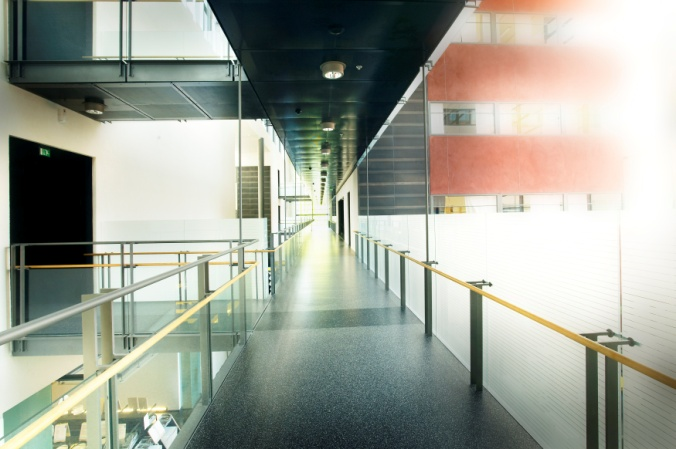
\includegraphics[width=8cm]{figures/arcada.jpg}
\caption{The interior of Arcada. Photograph Valtteri Kantanen Arcada 2008}
\end{figure}

\kant[2]

\cleardoublepage

\input{3-Methodology}
\cleardoublepage

\input{4-Experiments}
\cleardoublepage

\input{5-Results}
\cleardoublepage
\input{6-Conclusions}


% Here is the bibliography
\cleardoublepage
\phantomsection
% Uncomment for Swedish
%\renewcommand{\bibname}{Källor}
\renewcommand{\bibname}{References}
%\bibliographystyle{apa}
\bibliographystyle{bibliography}
\bibliography{7-references}



%\renewcommand{\bibname}{References}
%\bibliographystyle{bibliography}
%\bibliography{7-references}
%\newpage
\cleardoublepage
\phantomsection
\input{8-Appendices}



\end{document} 
